\chapter{Experiments and results}
\label{chap:experiments_and_results}


	% --- META INFO START: ---

	\besk{Et kapittel der du har satt opp (med hyper-parametere og miljø-variabler f.eks. i en oversiktlig tabell) eksperimenter, kjørt simulation-runs med disse verdiene, og viser hva resultatene ble. Resultater kan være \textbf{performance plot}s (ift. harmonic synch.-times for diverse hyper-parametere og miljøvariabler (samt om robotene er homogene eller heterogene og isåfall hvordan), der plottet må lages spesifikt for hvert eksperiment, og kan f.eks. være boxplot eller tabeller med performance-/hsynchtime-/simulation-time(s)-verdier), \textbf{harmonic synchrony detection plot}s (altså hvordan harmonic synch. ble detectet i et simulation-run), \textbf{phase-\&frequency-plot}s (altså hvilke fase- og frekvens-verdier robotene hadde iløpet av simulation-run'et, via \textit{plot\_PhaseFrequencyPlot\_for\_SimRun.py}), eller \textbf{synchrony-evolution plot}s (der 'towards\_k\_counter'en iløpet av simulation-run'et plottes, via \textit{plot\_SynchronyEvolutionPlot\_for\_SimRun.py})}

	\besk{Helst gode eksperimenter som motiveres og forklares, settes opp, og utføres m/resultater man diskuterer og analyserer. Det er bra å evaluere fra flere synspunkt \tcol[gray]{med flere research methods og hvis tid}}

	% --- META INFO STOP. ---


This chapter presents the experiments set up and performed in the novel synchronization simulator in Unity, as presented in Chapter \ref{chap:implementation}, for certain configurations of musical robot collectives. Effects of the individual musical robots's hyperparameters on the collective achievement and performance of achieving harmonic synchrony are presented. Some examples are hyperparameters which determines how much each musical robot will adjust itself after hearing a transmitted fire signal from a neighbouring robot; $\alpha$ for phase adjustment and $\beta$ for frequency adjustment.

The main performance scores presented in this chapter will consist of synchronization times given in simulation time (s) (i.e. how long it takes robot collectives to reach the state of harmonic synchrony if they ever do), accompanied by the respective and corresponding error rates during the belonging simulation runs (i.e. the percentage of robot collectives out of e.g. 30 runs failing to reach harmonic synchrony before the maximum time limit of e.g. 5 simulation minutes). If a musical robot collective then never reaches the target state of harmonic synchrony within the maximum time limit, this simulation run will be regarded as a ``synchronization fail'', and we will then not regard its termination time (in simulation time seconds) as \textit{harmonic synchronization time}—but simply that, that simulation run's termination time.



\section{Phase synchronization}
This is the section where experiments attempting to synchronize for the first and simpler problem, namely synchronizing only the phases $\phi_i$ of all agents $i$, are presented and analyzed resuls for. These are then experiments where all musical robots have an equal and fixed frequency, only adjusting phases, in order to entrain to synchronize their phases to each other until reaching the target state of harmonic synchrony.
	
	\subsection{Reproducing baseline results}
	
	In order to see that our developed synchronization simulator in Unity yields more or less the same results as Nymoen's results, similar experiments as reported in their paper are performed here. These tell us whether differences in performance, in terms of synchronization times (sim s), is simply due to implementation differences, or actually because of the utilized synchronization methods and hyperparameters in question. 
	
	First off, Mirollo \& Strogatz's phase adjustment method (as presented in \ref{mirollo_strogatz_phase_adjust}) is experimented with for the initial phase ($\phi$) synchronization problem, for varying phase coupling constants $\alpha$. Hyperparameters are set in the simulator as shown in Table \ref{tab:baseline_reproducing_phase_sync_for_alpha}. Results can be seen in Figure \ref{fig:baseline_reproducing_phase_sync_for_alpha}.
	
	\begin{center}
	\begin{tabular}{ |c|c|c|c|c|c|c| } 
	\hline
	$|R|$ & $\beta$ & $t_{ref}$ & $t_f$ & $k$ & $t_{max}$ \\
	\hline
	6 & 0 & 50ms & 80ms & 8 & 5min \\
	\hline
	\end{tabular}
	\captionof{table}{Experiment hyperparameter setup}
	\label{tab:baseline_reproducing_phase_sync_for_alpha}
	\end{center}
	
	\begin{figure}[ht!]
		\centering
		\includegraphics[width=\linewidth]{Assets/DocSegments/Chapters/ExperimentsAndResults/Figures/PerfScores/baseline_reproducing_phase_sync_for_alpha.pdf}
		\caption{Harmonic synchronization times (s) for 6 robots with initially random and unsynchronized phases but equal and fixed frequencies (1Hz), for varying phase coupling constants $\alpha$. 30 simulation runs per $\alpha$ are reported.}
		\label{fig:baseline_reproducing_phase_sync_for_alpha}
	\end{figure}
	
	
	\subsection{Hyperparameter tuning}
	
	Here we tune the hyperparameters $\alpha$ and $t_{ref}^{dyn}$ for several robot collective sizes, according to performance scores of how long it takes robot collectives on average to achieve harmonic synchrony. Exactly these two specific hyperparameters are experimented with mostly since they empirically seem to be the most important ones to set correctly before starting the simulator; that is, in order for the robots to actually manage achieving harmonic synchrony. Additionaly, the point of K. Konishi and H. Kokame (cf. \ref{sim_env_and_hyperparams}) was also remembered.
	
	The specific values of hyperparameters to test synchronization times for were chosen based on an initial and identical but failed experiment (not reported) where the tested values for $t_{ref}^{dyn}$ were showing some interesting effects for various robot collective sizes. Simple and limited insight was also collected from trial and error in the complete beginning when trying to facilitate stable and successful simulation runs. And furthermore, after seeing results found in this thesis for $\alpha$ already, we also got some more ideas for which values of $\alpha$ could be interesting to investigate further.
	
	Other constant hyperparameters not being tuned or experimented for in this experiment are shown in Table \ref{tab:exp_phase_sync_hyperparam_tuning}. The hyperparameter tuning results, where the effects of tuning hyperparameters $\alpha$ and $t_{ref}^{dyn}$ for various musical robot collective sizes, are shown in Figure \ref{fig:phase_sync_hyperparam_tuning_experiment}. Again, since we are synchronizing for the phase ($\phi$) synchronization problem, now only phases are initially unsynchronized, and frequencies are fixed and constant (1Hz) throughout the simulation runs.
	
	\begin{center}
	\begin{tabular}{ |c|c|c|c|c| } 
	\hline
	$\beta$ & $t_f$ & $k$ & $t_{max}$ \\
	\hline
	0 & 80ms & 8 & 5min \\
	\hline
	\end{tabular}
	\captionof{table}{Experiment hyperparameter setup}
	\label{tab:exp_phase_sync_hyperparam_tuning}
	\end{center}
	
	\begin{figure}[ht!]
	  \begin{subfigure}[b]{0.5\textwidth}
		\centering\captionsetup{width=.9\linewidth}%
		\includegraphics[width=\textwidth]{Assets/DocSegments/Chapters/ExperimentsAndResults/Figures/PerfScores/t_ref_dyn_x_alpha_hyperparamtuning_experiment_plot_collsize3.pdf}
		\caption{robot collective size $|R|$ = 3.}
		\label{fig:sub:t_ref_dyn_x_alpha_collsize3}
	  \end{subfigure}
	  %
	  \begin{subfigure}[b]{0.5\textwidth}
		\centering\captionsetup{width=.9\linewidth}%
		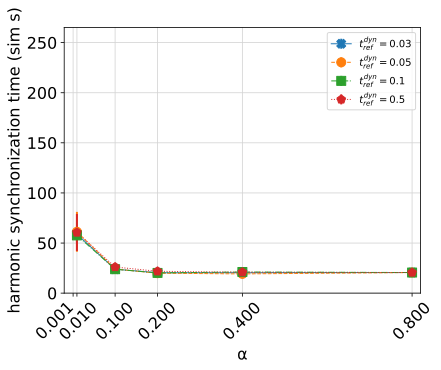
\includegraphics[width=\textwidth]{Assets/DocSegments/Chapters/ExperimentsAndResults/Figures/PerfScores/t_ref_dyn_x_alpha_hyperparamtuning_experiment_plot_collsize10.pdf}
		\caption{robot collective size $|R|$ = 10.}
		\label{fig:sub:t_ref_dyn_x_alpha_collsize10}
	  \end{subfigure}
	  \begin{subfigure}[b]{0.5\textwidth}
		\centering\captionsetup{width=.9\linewidth}%
		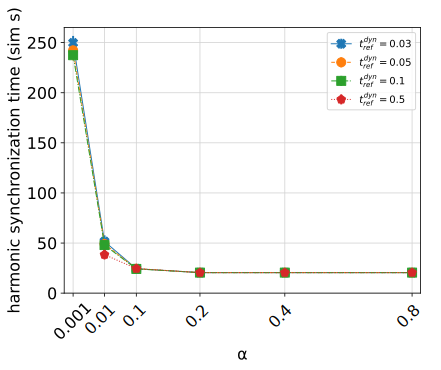
\includegraphics[width=\textwidth]{Assets/DocSegments/Chapters/ExperimentsAndResults/Figures/PerfScores/t_ref_dyn_x_alpha_hyperparamtuning_experiment_plot_collsize25.pdf}
		\caption{robot collective size $|R|$ = 25.}
		\label{fig:sub:t_ref_dyn_x_alpha_collsize25}
	  \end{subfigure}
	  %
	  \begin{subfigure}[b]{0.5\textwidth}
		\centering\captionsetup{width=.9\linewidth}%
		\includegraphics[width=\textwidth]{Assets/DocSegments/Chapters/ExperimentsAndResults/Figures/PerfScores/t_ref_dyn_x_alpha_hyperparamtuning_experiment_plot_collsize50.pdf}
		\caption{robot collective size $|R|$ = 50.}
		\label{fig:sub:t_ref_dyn_x_alpha_collsize50}
	  \end{subfigure}
	  \caption{Average harmonic synchronization times are plotted in errorbar plots, where the standard deviation is the error. 30 simulation runs per $\alpha$ and $t_{ref}^{dyn}$ pair are reported, unless simulation runs ended up as ``synchronization fails''.}
	  \label{fig:phase_sync_hyperparam_tuning_experiment}
	\end{figure}
	
	As we can see, there are generally low standard deviations which make errors in the plots barely visible. We also can notice that the largest differences are seen for lower $\alpha$ values, as average harmonic synchronization times are more and more overlapping and similar for larger $\alpha$ values.
	
	A general pattern we can see is that larger robot collective sizes (larger $|R|$ values) handle lower phase coupling constants $\alpha$ better; in that the music collectives both achieve harmonic synchrony in lower average times than the smaller robot collectives, as well as achieving lower error rates. To this latter point, note that for the lowest $\alpha$ value of 0.001, robot collectives with size $|R|=3$ and 10 were not able to achieve harmonic synchrony at all during any of the simulation runs (i.e. having 100\% error rate), whereas larger collective sizes like $|R|=25$ and $|R|=50$ managed to achieve harmonic synchrony despite the low $\alpha$ value. The reason for this can very well lie in the fact that, as we remember, the phase coupling constant $\alpha$ represents how much each robot will adjust its oscillator phase when hearing a ''fire`` signal from a neighbouring robot. If there are more neighbours firing ``adjustment signals'' to a certain robot (i.e. we have a higher collective size $|R|$), it is also logical that the robot in question will update its phase more often. And so we can then see why e.g. all average harmonic synchronization times for $\alpha=0.01$ seem to improve (i.e. gets reduced) for every increase in collective size $|R|$; the phase coupling constant $\alpha=0.01$ might be weak, but with further and more frequent weak adjustments accumulated over the same time, the weak $\alpha$ is compensated for.
	
	Hence, it seems like larger robot collectives do not require as large of a phase coupling constant $\alpha$ in order to synchronize to each other compared to that which smaller robot collectives require.
	
	
	\subsection{Comparing phase adjustment methods}
	So far in this chapter and section, we have only run experiments for pure phase synchronization, the $\phi$ problem, with Mirollo-Strogatz's method of phase adjustment, like described in \ref{mirollo_strogatz_phase_adjust}. With this method of phase synchronization, robots are simply adjusting phases in an excitatory way; they only ``push'' other ocillators's phases further or higher when firing themselves, never ``holding'' or ``dragging'' them back.
	
	Now, in order to investigate the validity of the claimed [] benefits of performing bi directional phase adjustments—both excitatory and inhibitory—like that of Nymoen's phase adjustment (see \ref{subsec:nymoen_phase_adjust}), an experiment comparing these two aforementioned phase adjustment methods thus follows.
	
	Empirically speaking based on previous results in phase synchronization experiments, in particular the ones shown in Figure \ref{fig:baseline_reproducing_phase_sync_for_alpha} and \ref{fig:phase_sync_hyperparam_tuning_experiment}, arguably the best values so far for $\alpha$ (i.e. $\alpha=0.8$) and $t_{ref}^{dyn}$ (i.e. $t_{ref}^{dyn}=0.1$) will be reused here for Mirollo-Strogatz's phase synchronization runs.
	
	Since we have not yet performed any experiments for pure phase synchronization in the $\phi$ problem using Nymoen's slightly modified and bi directional phase adjustment function, the same $\alpha$ value of 0.8 will also be used for the phase synchronization runs here.
	
	See the hyperparameter setup below in Table \ref{tab:directional_phase_adjustment_comparison}, and the results for the two phase adjustment methods given various robot collective sizes $|R|$ in \ref{}.
	
	\begin{center}
	\begin{tabular}{ |c|c|c|c|c|c|c| } 
	\hline
	$\alpha$ & $\beta$ & $t_{ref}^{dyn}$ & $t_f$ & $k$ & $t_{max}$ \\
	\hline
	0.8 & 0 & 10\% & 80ms & 8 & 5min \\
	\hline
	\end{tabular}
	\captionof{table}{Experiment hyperparameter setup}
	\label{tab:directional_phase_adjustment_comparison}
	\end{center}
	
	\tcol[blue]{FYLL INN}
	% GAMMEL EPA1-CAPTION: Performance-plot: harmonic synchronization-times from initial simulator-experiment when synchronizing phases $\phi_i$ for all agents $i$, where all phases are initially uniformly randomized between 0 and 1, and eventually synchronize and align. We here measure how long it takes 6 agents to synchronize their phases to each other, given the two different phase-adjustment methods. 30 individual runs per phase-adjustment method were performed in Unity for a collective-size of 6 agents, and $\alpha=0.2$ e.g.
	
% --- \section END. ---



\section{Phase and frequency synchronization}
This is the section for the experiments attempting to synchronize for the second and harder problem of synchronizing both phases $\phi_i$, as well as frequencies $\omega_i$, for all agents $i$. These are then experiments where all musical robots originally have unequal and ever-changing phases  and frequencies, adjusting both phases and frequencies in order to entrain to synchronize their phases and frequencies until reaching harmonic synchrony.

	\subsection{Reproducing baseline results}
	Again, we want to here see whether we get more or less the same results in the Unity simulator as K. Nymoen et al. get in their firefly oscillator system.
	
	Hence, we here present attempts made in the novel Unity synchronization simulator at recreating K. Nymoen et al.'s first results with their novel frequency synchronization method, which is utilizing, amongst other aspects, self awareness \cite{nymoen_synch}.
	
		\paragraph{Ordering by phase couplings}
		
		Given that K. Nymoen et al. do not mention their $\beta$ value in their frequency synchronization experiment where they order for different phase coupling values $\alpha$, an \textit{empirically decent} $\beta$ value of 0.4 is chosen for this experiment. What \textit{empirically decent} refers to in this case are K. Nymoen et al.'s findings in the results of their last experiment \cite{nymoen_synch} where synchronization times for various $\beta$ values were evaluated; deeming $\beta=0.4$ to be a good value, with no further improvement in synchronization performance when $\beta$ is increased further.
		
		Here, K. Nymoen et al.'s self aware frequency adjustment method, implemented in our novel synchrony simulator in Unity, is experimented with for varying phase coupling constants $\alpha$. This time not only oscillator phases are initially unsynchronized; oscillator frequencies are also unsynchronized to begin with. Hence, we here try to synchronize our musical robots in the phase ($\phi$) \textit{and} frequency ($\omega$) synchronization problem, using Nymoen's phase adjustment method to synchronize phases, as well as Nymoen's frequency adjustment method to synchronize frequencies. See set up hyperparameters in Table \ref{tab:baseline_reproducing_phase_and_freq_sync_for_alpha}. See the results in Figure \ref{fig:baseline_reproducing_phase_and_freq_sync_for_alpha}.
		
		\begin{center}
		\begin{tabular}{ |c|c|c|c|c|c|c|c|c|c| } 
		\hline
		$|R|$ & $\beta$ & $\omega_{min}^{init}$ & $\omega_{max}^{init}$ & $m$ & $t_{ref}$ & $t_f$ & $k$ & $t_{max}$ \\
		\hline
		6 & 0.4 & 0.5Hz & 4Hz & 5 & 50ms & 80ms & 8 & 5min \\
		\hline
		\end{tabular}
		\captionof{table}{Experiment hyperparameter setup}
		\label{tab:baseline_reproducing_phase_and_freq_sync_for_alpha}
		\end{center}
		
		\begin{figure}[ht!]
			\centering
			\includegraphics[width=\linewidth]{Assets/DocSegments/Chapters/ExperimentsAndResults/Figures/PerfScores/baseline_reproducing_phase_and_freq_sync_for_alpha.pdf}
			\caption{Harmonic synchronization times (sim s) for 6 robots with both initially unsynchronized phases \textit{and} frequencies, for varying phase coupling constants $\alpha$, reaching harmonic synchrony—but also often failing to. 30 simulation runs per $\alpha$ are reported.}
			\label{fig:baseline_reproducing_phase_and_freq_sync_for_alpha}
		\end{figure}
		
		
		\paragraph{Ordering by phase couplings but with more stable hyperparameters}
		
		When seeing how poorly the robot collectives managed to achieve harmonic synchrony in experiment [], we change the hyperparameters slightly in the hopes of achieving harmonic synchrony more frequently, or in other words more stable synchronization simulation runs. The reason is mostly that it would be beneficial to actually see whether we observe similar patterns as in Nymoen's results—something which becomes impossible when robot collectives nearly never achieve harmonic synchrony.
		
		The frequency coupling constant of $\beta=0.6$ could potentially be another supposed good $\beta$ value, at least solely judging by Nomoen's results, and hence we select this value for this hopefully stable phase and frequency synchronization experiment.
		
		By initial trial and error, it also became apparent that phase \textit{and} frequency synchronization was not always stable—i.e. the robot collective not managing to achieve harmonic synchrony within the maximum time limit—for collective sizes of 6 or more. It did however become apparent that phase \textit{and} frequency synchronization \textit{was} stable for smaller musical robot collective sizes, like 2 or 3.
		
		Hence, a similar experiment to as in [] is set up in the Unity synchrony simulator, and is run similarly as before. So still, the phase ($\phi$) \textit{and} frequency ($\omega$) synchronization problem is to be experimented for, given different phase coupling constants $\alpha$, with Nymoen's both phase and frequency adjustment methods—only this time with $\beta=0.6$ and $collsize=3$ instead. See set up hyperparameters in Table \ref{tab:stable_baseline_reproducing_phase_and_freq_sync_for_alpha}. See results in Figure \ref{fig:stable_baseline_reproducing_phase_and_freq_sync_for_alpha}.
		
		\begin{center}
		\begin{tabular}{ |c|c|c|c|c|c|c|c|c|c| } 
		\hline
		$|R|$ & $\beta$ & $\omega_{min}^{init}$ & $\omega_{max}^{init}$ & $m$ & $t_{ref}$ & $t_f$ & $k$ & $t_{max}$ \\
		\hline
		3 & 0.6 & 0.5Hz & 4Hz & 5 & 50ms & 80ms & 8 & 5min \\
		\hline
		\end{tabular}
		\captionof{table}{Experiment hyperparameter setup}
		\label{tab:stable_baseline_reproducing_phase_and_freq_sync_for_alpha}
		\end{center}
		
		\begin{figure}[ht!]
			\centering
			\includegraphics[width=\linewidth]{Assets/DocSegments/Chapters/ExperimentsAndResults/Figures/PerfScores/stable_baseline_reproducing_phase_and_freq_sync_for_alpha.pdf}
			\caption{Harmonic synchronization times (sim s) for 3 robots with both initially unsynchronized phases \textit{and} frequencies for varying phase coupling constants $\alpha$. 30 simulation runs per $\alpha$ are reported.}
			\label{fig:stable_baseline_reproducing_phase_and_freq_sync_for_alpha}
		\end{figure}
		
	
		\paragraph{Ordering by frequency couplings}
		
		\tcol{ Now, we perform the same phase \& frequency synchronization experiment as in Figure \ref{fig:exp2}, except that this time we will fix the phase coupling constant $\alpha$ and instead test how the individual musical robots's various frequency coupling constants $\beta$ affect the performance of the musical robot collective. These results are shown in Figure \ref{fig:exp3} }
		
		\tcol{ Again, K. Nymoen et al. does not specify exactly the phase coupling constant they use in this latter experiment when testing their firefly-inspired synchronization system for various $\beta$ values. Hence, the now fixed phase coupling constant $\alpha$ is here selected by reusing the $\alpha$ value found in the similar experiment presented in Figure \ref{fig:exp3} to yield the lowest error rate in the musical robot collective when synchronizing to each other. This then gives us a fixed $\alpha = 0.2$. If we also survey the harmonic synchronization times and error rates in the other experiments presented in the thesis, we can also see that a phase coupling constant $\alpha=2$ should be among the best values we could use. }
		
		See the set up hyperparameters for the experiment in Table \ref{tab:baseline_reproducing_phase_and_freq_sync_for_beta}, and the corresponding results in Figure \ref{fig:baseline_reproducing_phase_and_freq_sync_for_beta}.
		
		\begin{center}
		\begin{tabular}{ |c|c|c|c|c|c|c|c|c|c| } 
		\hline
		$|R|$ & $\alpha$ & $\omega_{min}^{init}$ & $\omega_{max}^{init}$ & $m$ & $t_{ref}$ & $t_f$ & $k$ & $t_{max}$ \\
		\hline
		6 & 0.2 & 0.5Hz & 4Hz & 5 & 50ms & 80ms & 8 & 5min \\
		\hline
		\end{tabular}
		\captionof{table}{Experiment hyperparameter setup}
		\label{tab:baseline_reproducing_phase_and_freq_sync_for_beta}
		\end{center}
		
		\begin{figure}[ht!]
			\centering
			\includegraphics[width=\linewidth]{Assets/DocSegments/Chapters/ExperimentsAndResults/Figures/PerfScores/baseline_reproducing_phase_and_freq_sync_for_beta.pdf}
			\caption{Synchronization times (s) for 6 robots with both initially random and unsynchronized phases, and frequencies, for varying frequency coupling constants $\beta$. 30 simulation runs per $\beta$ are reported.}
			\label{fig:baseline_reproducing_phase_and_freq_sync_for_beta}
		\end{figure}
		
		Even though we do not see exactly the same harmonic synchronization times as we see in Nymoen's results, and worse at that, we do in fact see a similar pattern in that also here, synchronization times and error scores seem to improve the larger frequency coupling constant $\beta$ we have.
		
		Also, from the results in Figure \ref{fig:phase_and_freq_sync_baseline_reproducing_experiment}, it becomes apparent that $\beta=0.7$ might be the best choice to continue using in our Unity synchrony simulator—at least when it comes to collective sizes of $|R|=6$.
		
	
	\subsection{Increasing degree of self awareness}
	
	It has previously, although more mathematically and not so much experimentally, been attempted to reduce the connectivity assumptions in pulse coupled oscillators \cite{minimally_connected_pcos} and to analyze the effects of it.
	
	Here the hypothesis of whether increasing musical robots's degrees of self awareness will affect the synchronization performance or not, is investigated experimentally. Exactly what is meant by an increasing degree of self awareness specifically refers to the robots's \textit{self awareness scope} \cite{sacs17_ch3}. This is tested in Unity for the more challenging $\phi \& \omega$ problem of harmonically synchronizing both phases and frequencies. Perhaps a larger self awareness scope, meaning more knowledge about the social environment, will lead to the robots having a better ``overview'' of the environment; hence leading to shorter simulation time (s) before reaching the goal state of harmonic synchrony. Or perhaps hearing more ``fire'' signals on average simply will be disturbing to the robots and hence disturb and slow down their entrainment towards harmonic synchrony. This experiments attempts to answer questions like these by for the following three scenarios evaluating collective synchronization performance:
	
	\begin{enumerate}
		\item \textbf{Minimal self awareness scope}: Each individual robot only hears the nearest neighbouring robot's ``fire'' signals []. In this case, robots have limited and more local knowledge.
		\item \textbf{Radial self awareness scope}: Each individual robot hears neigbouring robots's ``fire'' signals within a radius $d$ around it []. In this case, robots have more knowledge but also still locally.
		\item \textbf{Global self awareness scope}: Each individual robot hears all other neigbouring robots's ``fire'' signals []. In this case, robots have maximum and global knowledge when it comes to awareness of other neighbouring robots.
	\end{enumerate}
	
	In this way, the degree to which robots are self aware of or communicating with other robots is increasing. The effects of increasing the degree of self awareness in this sense are shown in [].
	
% --- \section END. ---